\documentclass[../../main.tex]{subfiles}

\begin{document}

\subsection{Class diagram}

A UML class diagram describing the main entities involved in the system follows.
Customers use the system to line up in the queue of a store and obtain a line up
receipt, which will grant them a visit to the store. Each store belongs to a given
chain of stores. Moreover, each store can be internally divided in departments,
containing different categories of purchasable items. When the customers line
up, they can specify the categories of items they intend to buy. Finally, the
system knows the locations of the customers and of the stores.

The line up receipt is represented by a QR code for the customers that interact with the system with an IT device.

If the customers interact with the system using a standard telephone line, they are given a numeric code as a representation of the line up receipt, which they will be able to convert to a printed QR code line up receipt thanks to the store assistants outside of the store.

The customers who interact with the system in presence request the printed QR code line up receipt directly to the store assistants outside of the store.

\begin{figure}[h!]
    \centering
    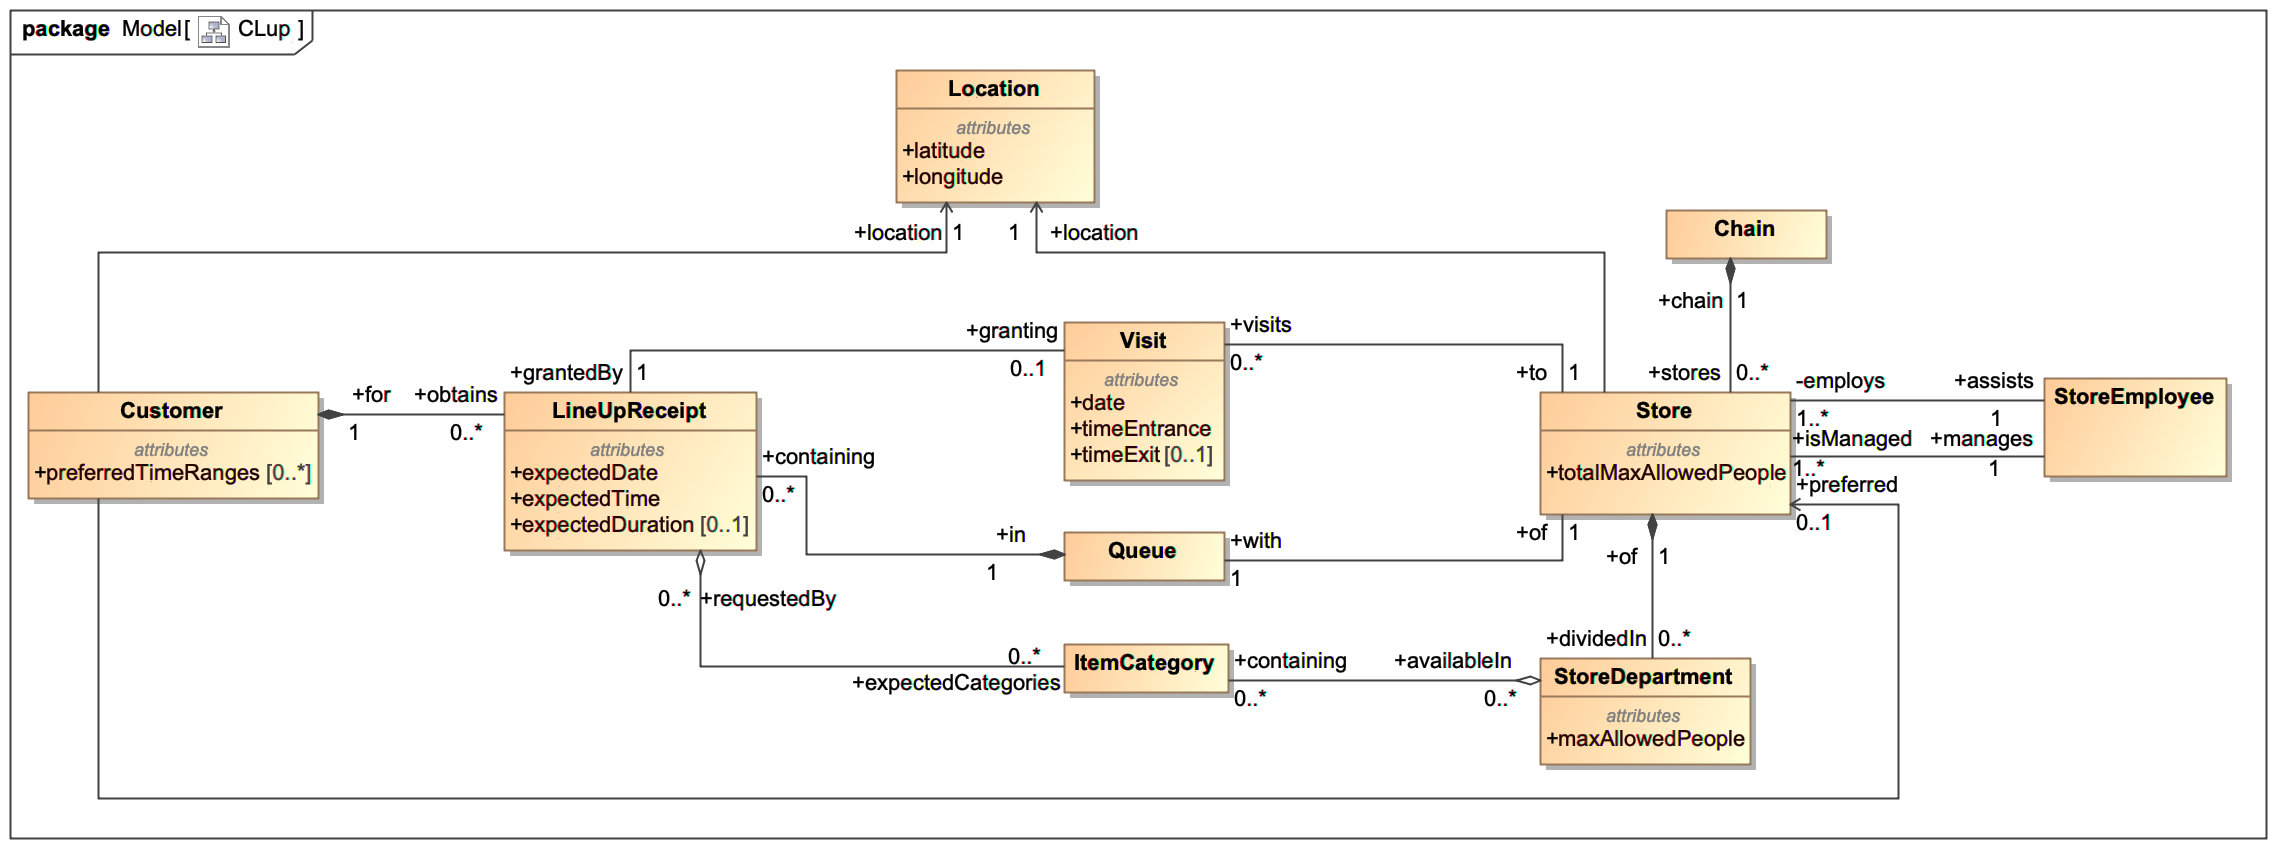
\includegraphics[width=\textwidth]{class__CLup.png}
    \caption{The class diagram of CLup's application domain.}
\end{figure}

\subsection{State chart diagrams}

The internal state of the main entities of the domain is better defined in the following UML
state diagrams.

\begin{figure}[h!]
    \centering
    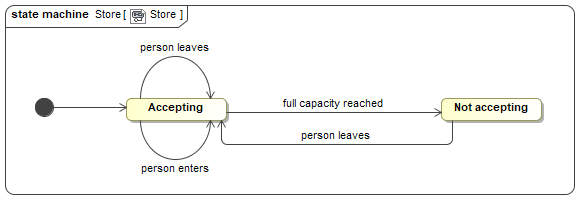
\includegraphics[width=\textwidth]{stm__Store__Store.png}
    \caption{Statechart of a store in the application domain.}
\end{figure}

\begin{figure}[h!]
    \centering
    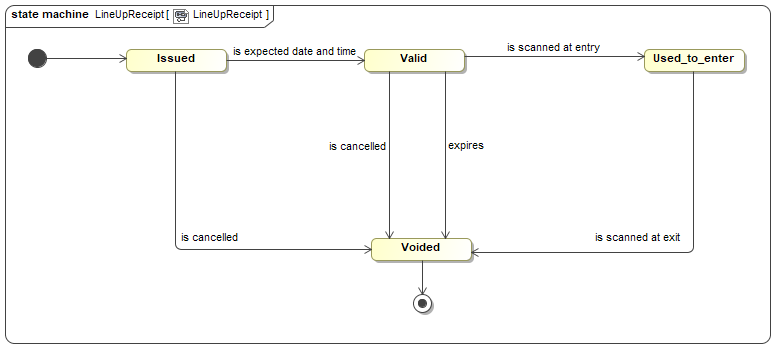
\includegraphics[width=\textwidth]{stm__LineUpReceipt__LineUpReceipt.png}
    \caption{Statechart of a lineup receipt in the application domain.}
\end{figure}

\end{document}
